\documentclass[pdf,aspectratio=169]{beamer}
\usepackage[]{hyperref,graphicx,siunitx,lmodern,booktabs,tikz,tensor}
\usepackage{pgfplots, pgfplotstable}
\usepackage{pdfpc-commands}
\usepackage[mode=buildnew]{standalone}
\mode<presentation>{\usetheme{Astro}}

\graphicspath{ {../Images/} }

\sisetup{per-mode=symbol}
\usetikzlibrary{calc,intersections, decorations.pathmorphing,shadings,shapes.geometric}
%\tikzstyle{proton}=[circle, minimum size = 7mm, ball color=red, black,transform shape]
%\tikzstyle{neutron}=[circle, minimum size=7mm, ball color=gray, black, transform shape]
%\tikzstyle{gammaray}=[ultra thick, -latex, decorate, decoration={snake, post length=3mm}]
\tikzstyle{image}=[inner sep=0pt, outer sep=0pt]


%preamble
\title{On Being Galactose Tolerant}
\date{November 26, 2018}
\author{Jed Rembold}

\begin{document}
\renewcommand*{\theenumi}{\Alph{enumi}}

\begin{frame}{Announcements}
  \begin{itemize}
	\item Webwork due on Wednesday!
	\item Group A: Last lab this week!
	\item Hopefully will hand back tests on Wednesday
	\item I'm pushing out new grade reports (with Test 3 results) today
	\item Polling: \url{rembold-class.ddns.net}
  \end{itemize}
\end{frame}

\begin{frame}{APOD!}
	\begin{center}
		%\includegraphics[width=0.8\textwidth]{APOD_RougeAsteroid.jpg}
		\begin{tikzpicture}
			\node[anchor=south east] at (0,0) {\inlineMovie{../Videos/RocketLaunch.ogv}{../Videos/RocketLaunch.png}{width=.8\textwidth}};
			\node[anchor=south east, draw, rounded corners, Orange, font=\scriptsize] at (-.2,.2) {\href{https://www.youtube.com/watch?v=B1R3dTdcpSU}{Link to Video}};
		\end{tikzpicture}
	\end{center}
\end{frame}

\begin{frame}{Review Question}
  You observe two Type II Cepheid variable stars to have the same peak apparent brightness from Earth. Star A has a period of 5 days and Star B has a period of 10 days. Which star is further from the Earth?
  \begin{enumerate}
	\item Star A
	\item \alert<2>{Star B}
	\item They are the same distance
	\item You can't say without knowing their temperatures
  \end{enumerate}
\end{frame}

\begin{frame}{It all takes shape\ldots}
  \begin{center}
	\includegraphics<1>[width=.7\textwidth]{ch15_MW_Top.png}
	\includegraphics<2>[width=.8\textwidth]{ch15_MW_Side.png}
  \end{center}
\end{frame}

\begin{frame}{Orbital Paths}
  \begin{center}
	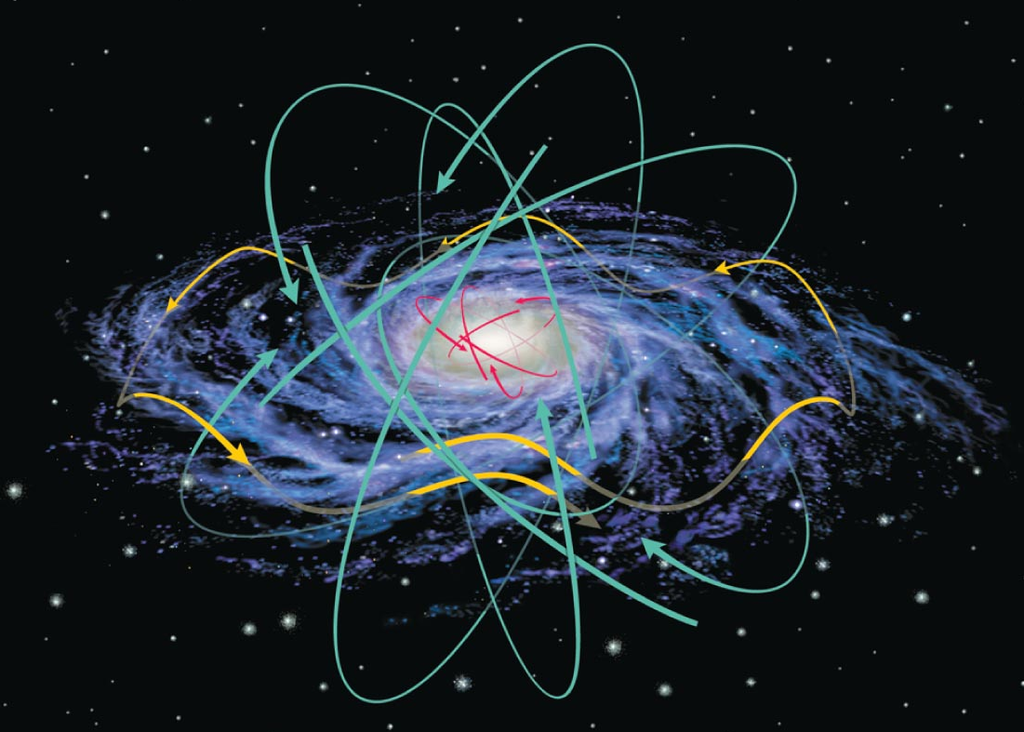
\includegraphics[width=.7\textwidth]{ch15_MW_StarMotions.png}
  \end{center}
  \begin{itemize}
	\item Disk stars move in circular paths + some up-down
	\item Halo stars move in large circles in all directions
	\item Bulge stars have some characteristics of both. More complicated.
  \end{itemize}
\end{frame}

\begin{frame}{The Scales Don't Lie}
  \begin{columns}
	\column{.5\textwidth}
	\begin{itemize}
	  \item By observing nearby stars, we know that we orbit the center of the Milky Way at about \SI{220}{\kilo\meter\per\second}
		\begin{itemize}
		  \item Gives an orbital period of about 230 million years
		\end{itemize}
	  \item We know the distance. We know the period.
		\begin{itemize}
		  \item Kepler's Third Law! (Newton's Form)
		  \item Gives a mass of about \SI{2e41}{\kilo\gram}
		\end{itemize}
	\end{itemize}
	\column{.5\textwidth}
	\begin{block}{Calculation!}
	  \begin{align*}
		\frac{P^2}{a^3} &= \frac{4\pi^2}{GM} \\
		\Rightarrow M &= \frac{4\pi^2 a^3}{G P^2} \\
		&= \frac{4\pi^2 \left(\SI{2.6e20}{\meter} \right)^3}{(\num{6.67e-11})(\SI{7.258e15}{\second})} \\
		&= \SI{1.97e41}{\kilo\gram}
	  \end{align*}
	\end{block}
  \end{columns}
\end{frame}

%\begin{frame}{A Conundrum!}
  %\begin{itemize}
	%\item Planet speeds drop away with distance from the Sun
	%\item We'd expect star speeds to drop away with distance from the center of the galxy
	  %\begin{center}
		%\pause
		%\textcolor{Red}{BUT THEY DON'T!}
	  %\end{center}
	  %\pause
	%\item Implies that all the mass isn't focused at the center, but more spread out
	%\item But there aren't stars in most of those areas!
	%\item Dark Matter?
	  %\begin{itemize}
		%\item Stay tuned for coming chapters!
	  %\end{itemize}
  %\end{itemize}
%\end{frame}

\begin{frame}{Where is all the Mass?}
  \begin{itemize}
	\item Most of the mass we know of in the universe (or galaxy) is in stars
	\item Most of the stars are near the center of the galaxy
	\item Rotation curves tell us differently however!
  \end{itemize}
  \begin{center}
	\includegraphics[width=.7\textwidth]{ch16_mw_visible.png}
  \end{center}
\end{frame}

\begin{frame}{Rotation Curves: Planets}
  \begin{center}
	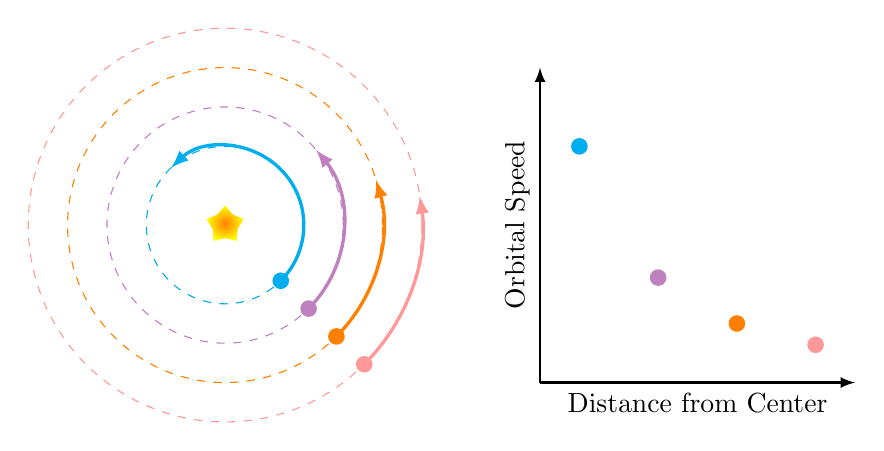
\begin{tikzpicture}
	  \coordinate (center) at (0,0);
	  \coordinate (origin) at (4,-2);

	  \node[star, inner color=orange, outer color=yellow] at (center) {};
	  \foreach \r/\c in {1/cyan, 1.5/violet!50, 2/orange, 2.5/red!40}{
		\draw[dashed, \c] (center) circle (\r);
		\coordinate (p) at ($(center)+(-45:\r)$);
		\fill[\c] (p) circle (3pt);
		\draw[very thick, -latex, \c] (p) arc (-45:{40/(.3*\r*\r*\r)}:\r);
	  }

	  \draw[-latex,thick] (origin) --+(0,4) node[midway,above,sloped] {Orbital Speed};
	  \draw[-latex,thick] (origin) --+(4,0) node[midway,below] {Distance from Center};
	  \foreach[count=\i] \r/\c in {1/cyan, 1.5/violet!50, 2/orange, 2.5/red!40}{
		\fill[\c] ($(origin)+(\i-.5,{3/(\r*\r)})$) circle (3pt);
	  }
	\end{tikzpicture}
  \end{center}
\end{frame}

\begin{frame}{Rotation Curves: Wheel}
  \begin{center}
	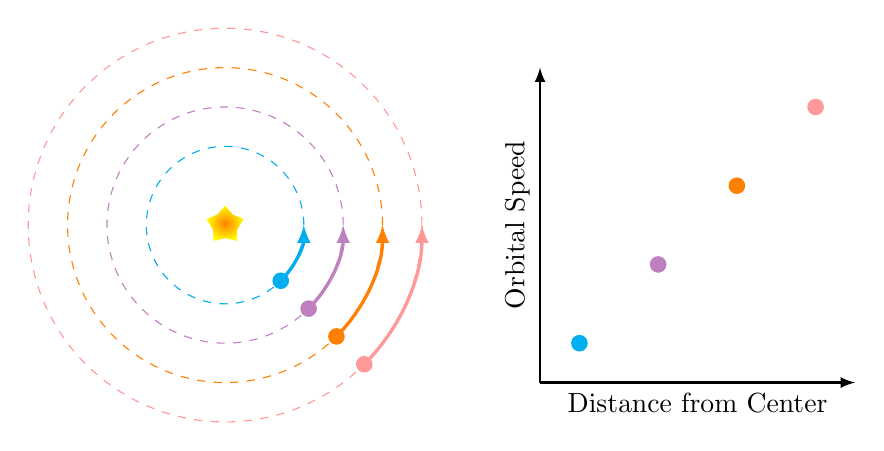
\begin{tikzpicture}
	  \coordinate (center) at (0,0);
	  \coordinate (origin) at (4,-2);

	  \node[star, inner color=orange, outer color=yellow] at (center) {};
	  \foreach \r/\c in {1/cyan, 1.5/violet!50, 2/orange, 2.5/red!40}{
		\draw[dashed, \c] (center) circle (\r);
		\coordinate (p) at ($(center)+(-45:\r)$);
		\fill[\c] (p) circle (3pt);
		\draw[very thick, -latex, \c] (p) arc (-45:0:\r);
	  }

	  \draw[-latex,thick] (origin) --+(0,4) node[midway,above,sloped] {Orbital Speed};
	  \draw[-latex,thick] (origin) --+(4,0) node[midway,below] {Distance from Center};
	  \foreach[count=\i] \r/\c in {1/cyan, 1.5/violet!50, 2/orange, 2.5/red!40}{
		\fill[\c] ($(origin)+(\i-.5,\i-.5)$) circle (3pt);
	  }
	\end{tikzpicture}
  \end{center}
\end{frame}

\begin{frame}{Rotation Curves: Milky Way}
  \begin{center}
	\begin{tikzpicture}
	  \begin{axis}[
		  width=\textwidth,
		  height=7cm,
		  xlabel=Distance from Center (in 1000 lyrs),
		  ylabel=Orbital Speed (km/s),
		]
		\addplot[only marks, violet!50] table[x index=0, y index=1] {../Data/MW_RotCurve.csv};
	  \end{axis}
	\end{tikzpicture}
  \end{center}
\end{frame}

\begin{frame}{Conclusions}
  \begin{columns}
	\column{.5\textwidth}
	\begin{itemize}
	  \item The Milky Way as a whole contains:
		\begin{itemize}
		  \item 5-10 times as much mass as can be seen at any wavelength
		  \item Spread throughout the galaxy and beyond
		\end{itemize}
	  \item Decidedly does NOT have the mass concentrated in the center
	\end{itemize}
	\column{.6\textwidth}
	\begin{center}
	  \begin{tikzpicture}
		\fill[black] (0,0) circle (3cm);
		\shade[inner color=black, outer color=Background, even odd rule] (0,0) circle (3cm) (0,0) circle (3.5cm);
		\shade[inner color=yellow, outer color=black, opacity=0.3] (0,0) circle (2cm);
		\fill[orange!50!yellow] (0,0) circle (3mm);
		\fill[orange!50!yellow] (0,0) ellipse (8mm and 1mm);
	  \end{tikzpicture}
	\end{center}
  \end{columns}
\end{frame}


\fullFrameImage{ch15_gas_cycle.png}

\begin{frame}{Reduce, Reuse, Recycle!}
  \begin{columns}
	\column{.5\textwidth}
	\begin{itemize}
	  \item We a pretty solid already with the star formation through lifetime side of things
	  \item What about the backside of the cycle?
		\begin{itemize}
		  \item Mainly a question of cooling
			\begin{itemize}
			  \item High speed gas from star outflows or explosions sweeps up ISM
			  \item Creates hot bubbles
			  \item Cool as they expand and run into surrounding ISM
			  \item Possible to ``blowout'' of the galactic disk
			\end{itemize}
		\end{itemize}
	\end{itemize}
	\column{.5\textwidth}
	\begin{center}
	  \begin{tikzpicture}[scale=1.4, transform shape]
		\clip[rounded corners] (0.1,.1) rectangle (4.9,4);
		\node[image, anchor=south west] at (0,0) {\includegraphics[width=5cm]{ch15_bubble_breaker.png}};
	  \end{tikzpicture}
	\end{center}
  \end{columns}
\end{frame}

\begin{frame}{Atomic Hydrogen}
  \begin{itemize}
	\item Further cooling causes the gas to become un-ionized
	\item Left with atomic hydrogen gas
	  \begin{itemize}
		\item Along with the normal mixture of helium and other trace elements
	  \end{itemize}
	\item Can ``see'' atomic hydrogen in Radio waves
	\item Gravity slows draws gas together into clumps
	  \begin{itemize}
		\item Radiate heat better, so they cool
		\item Form molecular clouds
	  \end{itemize}
	\item And the process repeats!
  \end{itemize}
\end{frame}

\begin{frame}{Seeing the Star-Gas-Star Cycle}
  \begin{itemize}
	\item Different wavelengths of light give us information on different points in the cycle!
	  \begin{itemize}
		\item \textcolor{Orange}{\SI{21}{\centi\meter} Radio} --  Shows atomic hydrogen gas
		\item \textcolor{Orange}{\SI{1.3}{\milli\meter} Radio} -- Shows molecular gas
		\item \textcolor{Orange}{\SI{90}{\micro\meter} Far Infrared} -- Shows dust
		\item \textcolor{Orange}{\SI{2}{\micro\meter} Near Infrared} -- Shows stars
		\item \textcolor{Orange}{\SI{650}{\nano\meter} Visible Light} -- Light emmitted and scattered
		\item \textcolor{Orange}{\SI{1.6}{\nano\meter} X-Ray} -- Hot gas bubbles and X-Ray binaries
		\item \textcolor{Orange}{\SI{10}{\pico\meter} Gamma Ray} -- Cosmic Ray collisions
	  \end{itemize}
  \end{itemize}
\end{frame}

\begin{frame}{Pretty Pictures!}
  \begin{center}
	\begin{tikzpicture}
	  \begin{scope}[scale=1.2, transform shape]
		\clip (0,0) ellipse (5cm and 2.5cm);
		\node[image] at (0,0) {\includegraphics[width=\textwidth]{ch15_mw_radio1.png}};
		\node<2>[image] at (0,0) {\includegraphics[width=\textwidth]{ch15_mw_radio2.png}};
		\node<3>[image] at (0,0) {\includegraphics[width=\textwidth]{ch15_mw_finfrared.png}};
		\node<4>[image] at (0,0) {\includegraphics[width=\textwidth]{ch15_mw_ninfrared.png}};
		\node<5>[image] at (0,0) {\includegraphics[width=\textwidth]{ch15_mw_visible.png}};
		\node<6>[image] at (0,0) {\includegraphics[width=\textwidth]{ch15_mw_xray.png}};
		\node<7>[image] at (0,0) {\includegraphics[width=\textwidth]{ch15_mw_gammaray.png}};
	  \end{scope}

	  \node<1> at (0,-3.5) {Atomic Hydrogen};
	  \node<2> at (0,-3.5) {Molecular Clouds};
	  \node<3> at (0,-3.5) {Interstellar Dust};
	  \node<4> at (0,-3.5) {Stars!};
	  \node<5> at (0,-3.5) {Our Visible View};
	  \node<6> at (0,-3.5) {Hot gases and X-ray binaries};
	  \node<7> at (0,-3.5) {Cosmic rays interacting with atomic nuclei};
	\end{tikzpicture}
  \end{center}
\end{frame}

%Magic command to have a top aligned shortstack (else the density line looked dumb)
\newcommand{\blap}[1]{\smash[b]{\begin{tabular}[t]{@{}c@{}}#1\end{tabular}}}

\begin{frame}{Phases of the ISM}
  \begin{center}
	\tiny
	\begin{tabular}[h!]{lp{1.2cm}rrp{2.5cm}}
	  \toprule
	  Gas State & Primary Component & Temperature & \blap{Density\\(atoms per cm$^3$)} & Description \\
	  \midrule
	  Hot Bubbles & Ionized hydrogen & \SI{1000000}{\kelvin} & 0.01 & Pockets of gas heated by supernova shock waves \\
	  Warm Atomic Gas & Atomic hydrogen & \SI{10000}{\kelvin} & 1 & Fills much of the galactic disk \\
	  Cool atomic clouds & Atomic hydrogen & \SI{100}{\kelvin} & 100 & Intermediate stage \\
	  Molecular clouds & Molecular hydrogen & \SI{30}{\kelvin} & 300 & Star forming regions\\
	  \bottomrule
	\end{tabular}
  \end{center}
  \begin{itemize}
	\item So temperature decreases as the cloud cools (duh)
	\item Density increases as the cloud cools
  \end{itemize}
\end{frame}

%\begin{frame}{Understanding Check}
  %Suppose you wanted to look to see if it is molecular clouds that block much of galaxy's starlight from reaching the Earth? What wavelengths would be most useful to observe in?
  %\begin{enumerate}
	%\item Infrared and X-ray
	%\item Near-Infrared and long wavelength radio
	%\item Visual and Near-Infrared
	%\item \alert<2>{Short wavelength radio and visual}
  %\end{enumerate}
%\end{frame}

\begin{frame}{Spiral Arms}
  \begin{columns}
	\column{.5\textwidth}
	\begin{itemize}
	  \item Bright blue regions indicate star forming regions
	  \item Galaxy rotates at same speed, so inner bits have shorter periods
	  \item If arms moved with stars, they would get all wound up!
	  \item Spiral Density Waves
		\begin{itemize}
		  \item Pinches everything together in that region
		  \item Doesn't effect normal stars much
		  \item Gives molecular clouds a chance to start star formation
		\end{itemize}
	\end{itemize}
	\column{.5\textwidth}
	\begin{center}
	  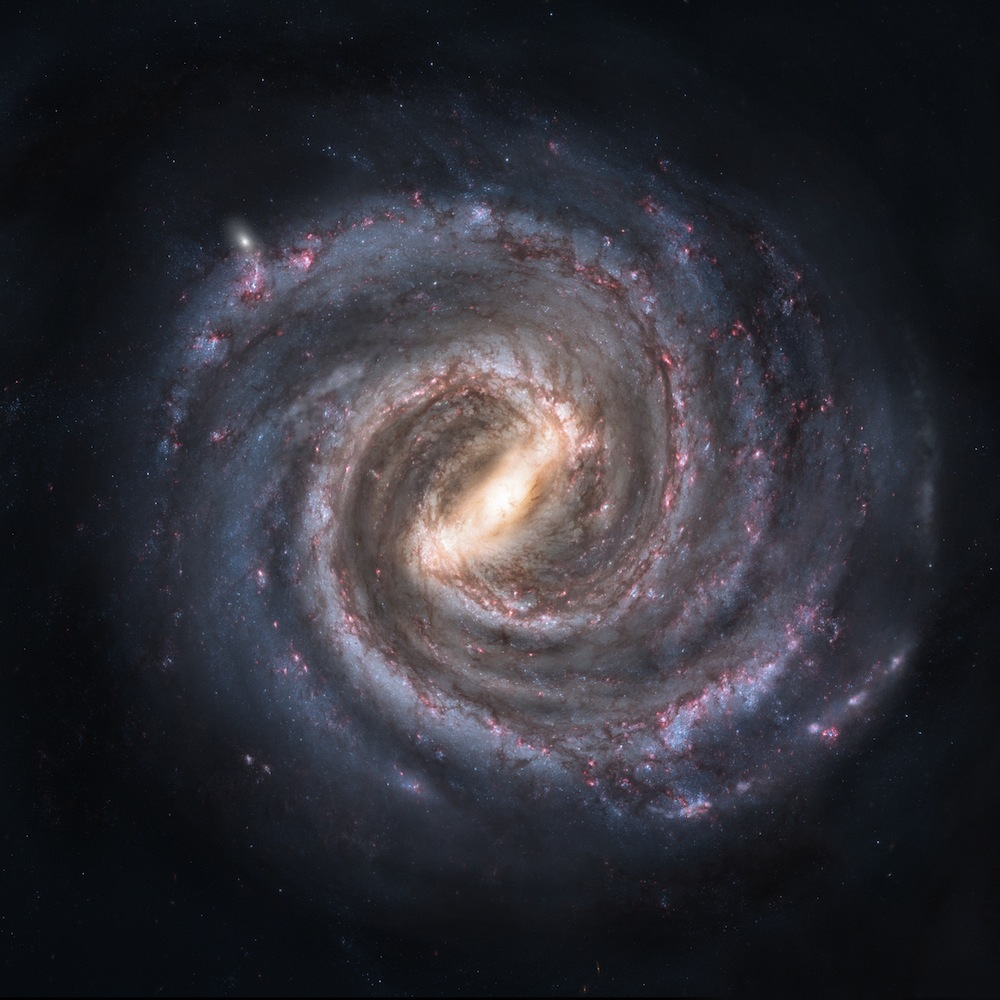
\includegraphics[width=.9\textwidth]{ch15_spiral_galaxy.jpg}
	\end{center}
  \end{columns}
\end{frame}

\begin{frame}{Regions of the Milky Way}
  \begin{itemize}
	\item The Disk
	  \begin{itemize}
		\item Younger generation of stars
		\item Contains gas and dust
		\item Location of open clusters
	  \end{itemize}
	\item The Bulge
	  \begin{itemize}
		\item Mixture of young and old stars
	  \end{itemize}
	\item The Halo
	  \begin{itemize}
		\item Older generation of stars
		\item Contains no gas or dust
		\item Location of globular clusters
	  \end{itemize}
  \end{itemize}
\end{frame}

%\begin{frame}{I can see your Halo}
  %\begin{itemize}
	%\item Stars in the Halo are old!
	  %\begin{itemize}
		%\item A smaller fraction of heavy elements than the Sun
		%\item Largely low-mass, red stars
	  %\end{itemize}
	%\item Stars in the disk are relatively young
	  %\begin{itemize}
		%\item A greater or equal fraction of heavy elements to the Sun
		%\item Lots of high and low mass stars, both blue and red
	  %\end{itemize}
	%\item Stars in the Halo must have formed \alert{early} in the Milky Way's history
	  %\begin{itemize}
		%\item When fewer heavy elements existed
		%\item No ISM (gas) in the halo
		%\item Star formation in halo stopped long ago when the gas got flattened into the disk
	  %\end{itemize}
  %\end{itemize}
%\end{frame}

%\begin{frame}{Galaxy Formation}
  %\begin{columns}
	%\column{.5\textwidth}
	%\begin{itemize}
	  %\item Any theory of galactic formation needs to predict these differences between halo and disk stars
	  %\item Going theory is that of a giant \alert{protogalactic cloud} that collapses
		%\begin{itemize}
		  %\item Halo stars form as it collapses
		  %\item Get left behind as angular momentum flattens the collapsing cloud
		%\end{itemize}
	%\end{itemize}
	%\column{.5\textwidth}
	%\begin{center}
	  %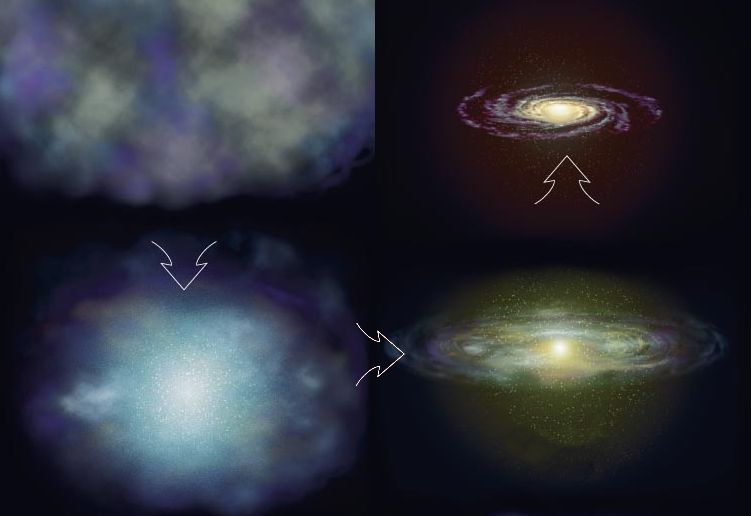
\includegraphics[width=\textwidth]{ch15_protogal_cloud.png}
	%\end{center}
  %\end{columns}
%\end{frame}

%\begin{frame}{Problems with Proto-Galactic clouds}
  %\begin{itemize}
	%\item Stars and star clusters should be forming the whole way through the stars collapse
	%\item So halo stars far from the center would be older than halo stars nearer to the center
	  %\begin{itemize}
		%\item Would imply that far away halo stars should have the least heavy elements
	  %\end{itemize}
	%\item But in truth ALL halo stars have the same elemental composition
	%\item Suggests a collision between multiple protogalactic clouds
  %\end{itemize}
%\end{frame}

%\begin{frame}{Galaxy Collisions}
  %\begin{columns}
	%\column{.4\textwidth}
	%\begin{itemize}
	  %\item Galaxies tend to cluster in groups
	  %\item Means collisions are a real possibility
	  %\item Milky Way has already consumed two galaxies in the past
	  %\item Will collide with the Andromeda galaxy in about 5 billion years
	%\end{itemize}
	%\column{.7\textwidth}
	%\begin{center}
	  %\inlineMovie{../Videos/Galaxy_Collision.ogv}{../Videos/Galaxy_Collision.png}{width=\textwidth}
	%\end{center}
  %\end{columns}
%\end{frame}

%\begin{frame}{The Beast at the Center}
  %\begin{itemize}
	%\item We can see into the core with radio, infrared, and X-ray telescopes
	%\item Near the center, we see a radio source named Sagittarius A*
	%\item Lots of stars VERY close with orbits that suggest Sgr A* has a huge mass
  %\end{itemize}
  %\begin{columns}[t]
	%\column{.5\textwidth}
	%\begin{itemize}
	  %\item Almost certainly a black hole
		%\begin{itemize}
		  %\item Yet odd in that it is not a strong x-ray source
		  %\item Occasional bright x-ray bursts
		  %\item Clumps of infalling material instead of a smooth stream?
		%\end{itemize}
	%\end{itemize}
	%\column{.4\textwidth}
	%\begin{center}
	  %\includegraphics[width=4.5cm]{ch15_bh_center.png}
	%\end{center}
  %\end{columns}
%\end{frame}

\end{document}
